\chapter{EL Schemas}
\label{chap:schemas}

% points to consider for introducing schemas:
% - we have roles and variables
% - we have composition
% - we have inheritance
% - we have rich semantics
% - we have rich temporal relations

%Generating ``commonsense'' knowledge for intelligent understanding and reasoning is a difficult, long-standing problem, whose scale challenges the capacity of any approach driven primarily by human input. Furthermore, approaches based on mining statistically repetitive patterns fail to produce the rich representations humans acquire, and fall far short of human efficiency in inducing knowledge from text.
In this chapter, I introduce a new framework for event knowledge representation, the \textbf{EL schema}, which is designed to allow complex schemas with rich, formal semantics to be learned from natural language text with few examples.
While most modern approaches to automated script learning (e.g.~\cite{chambers2011ACL,pichotta2016WS,yuan2018OEP}) learn linear sequences of simple tuple representations of events, EL schemas are represented using formulas in an expressive formal logic.
EL schemas are collections of EL formulas, and allow for an unlimited number of participating entities, represented as variables which may be used throughout the schema.
These variables may be assigned types by using noun and adjective predications, and they may be related to one another using $n$-place predications.
EL schemas comprise multiple steps, which may be related with a powerful temporal algebra.
They are also recursively hierarchical structures; they may be nested as steps in other schemas. EL schemas are designed to naturally support inference about novel events on the basis of partial matches of observed formulas to known schemas, allowing the schema system to ``fill in the gaps''.
Their variables may be filled in by matching entities or steps from a story with entities or steps in a schema and making the relevant variable substitutions in all other schema components; the schema components that were not matched, but which had their variables bound, can be interpreted as inferences about the matched context.

The remainder of this chapter describes the structure and meaning of individual EL schemas (Section~\ref{sec:schema_def}); describes the two hierarchical models under which EL schemas may be organized (Section~\ref{sec:schema_hier}); discusses the formal semantic interpretation of EL schemas and the inference and learning systems surrounding them (Section~\ref{sec:formal_semantics}); introduces the notion of \textit{protoschemas}, and their role in the bottom-up EL schema learning process (Section~\ref{sec:protoschemas}); and outlines the matching of EL schemas to text and the drawing of inferences from those matches (Section~\ref{sec:match_inf}).

%allows for typed and interrelated participating entities; multiple temporally related subevents; specification of goals, preconditions, and postconditions; and nesting of subschemas as steps in another schema.


% Unlike the slot-and-filler structures often used in knowledge harvesting, this logical form allows us to specify complex relations and constraints over the slots. Though formal, the representations are language-like, and as such readily relatable to NL text. The agents, objects, and other roles in the schemas are represented by typed variables, and the event variables can be related through partial temporal ordering and causal relations.

%Past approaches to statistical schema learning have largely represented schemas as sequences of lexical event tuples \citep{chambers2008unsupervised,pichotta2016learning}. Seeking a richer representation, we adopt the rich, EL-based schema framework presented by \citet{Lawley2021LearningGE}, henceforth referred to in this paper as \textit{EL schemas}. EL schemas are section-based: the main two sections, \texttt{STEPS} and \texttt{ROLES}, enumerate the temporal events (``steps'') that make up the schema, and the type and relational constraints on the schema's participants, respectively (see Figure~\ref{fig:singleschema}).

%Designed as a suitable representation of human-centric events, EL schemas can also specify preconditions, postconditions, arbitrary temporal relationships between steps, and the \textit{goals} of individual participants in the schema. All schema participants are represented as typed variables, all sharing a scope within the same schema, and formulas may include any number of variables as arguments. EL schemas also allow for recursive \textit{nesting}: a schema may be embedded as a step in another schema, and implicitly expanded to check constraints or generate inferences.

%Our schema representation allows for features absent in other schema systems. Like Minsky's frames \citep{minsky1974MIT}, we can specify typed slots---e.g. \el{!r1 (?x agent6.n)}---but unlike most descendants of Minsky's frames, we can \textit{relate} slots with arbitrary logical formulas, e.g. \el{(not (?x (can.md (do2.v ?a2))))}. Like Schank and Abelson's scripts, we can specify temporal event sequences, and organize them hierarchically---but unlike Schank and Abelson's scripts, our verb predicates do not rely on an atomic set of primitive actions; their semantics may be specified freely, in terms of other schemas, information extracted from dictionary definitions, or even relevant physical simulations, if desired. They may also remain largely unspecified, or specified only in terms of their relationship to other words; not every word needs to be understood in all its aspects in order to learn useful schemas.



% \section{Protoschema Identification as FrameNet Parsing}

%\section{Latent Schema Sampling}

%\section{Schema Generalization}

\section{Schema Components}
EL schemas are rich, hierarchical data structures composed primarily of a set of EL \textbf{formulas} organized into one of several disjoint, named \textbf{sections}.
Each formula has a section-dependent \textbf{formula ID} to uniquely identify it within the scope of the schema.
Each schema also has a \textbf{header}: an EL proposition, and an episode characterized by the proposition, which names and summarizes the entire schema. 
Each header has a unique verb predicate at its core, and its arguments are variables defined and typed within the scope of the schema.
The header can be used to ``embed'' a schema as a step in another schema---in fact, each step in Figure~\ref{fig:libschema} is a header for an embedded schema---or it can be matched directly to a proposition in a story to automatically invoke the schema.

\begin{figure}
    \centering
    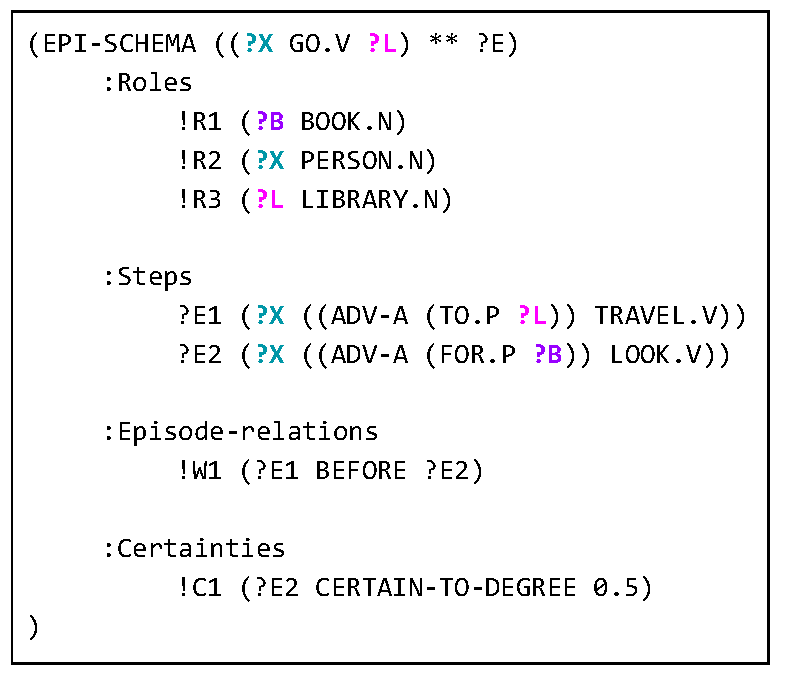
\includegraphics[width=0.65\columnwidth]{CH3_schemas/egschema.pdf}
    \caption{An example of a schema for a person going to a library.}
    \label{fig:libschema}
\end{figure}

\subsection{Formulas and Sections}
% Introduce formulas and discuss their piecewiseness
% Introduce formula-section layout
Schemas organize their constituent formulas in two types of sections: \textit{fluent} and \textit{nonfluent} sections. Nonfluent sections contain formulas that hold true regardless of time, and are marked by formula IDs beginning with exclamation marks. Such formulas include type constraints on entities (Section~\ref{sec:roles}), temporal relation predications on episodes (Section~\ref{sec:eprels}), and equality constraints on variables within subordinate schemas (Section~\ref{sec:scoping}). Fluent sections, on the other hand, contain formulas identified by variables starting with question marks; the truth value of these formulas is susceptible to change over time alone. Referring to the EL ontology in Figure~\ref{fig:el_ontology}, the semantic type of fluent predicates can be thought of as the more restrictive $(\mathcal{D}^{n} \rightarrow (\mathcal{M} \rightarrow \textbf{2}))$, rather than $(\mathcal{D}^{n} \rightarrow (\mathcal{S} \rightarrow \textbf{2}))$, as specific \textit{moments of time} ($\mathcal{M}$) are needed to determine truth value. Formally, a fluent formula $\phi$ with episode ID \el{?E} is said to characterize its episode ID: ($\phi ** \texttt{?E}$). A non-fluent formula $\psi$, however, does not have an episode ID, as its truth value is not temporally constrained; instead, it is represented by a \textit{metavariable} \el{!E}, any occurrence of which in an EL formula may be equivalently \textit{substituted} with $\psi$.

\subsection{Steps}
\label{sec:steps}
% steps of a schema are assumed to be linear unless eprels contradicts
% conjunctions are split up, XOR splits schema, splitting OR is OK depending on what semantics you want matching to have
% implicit relations to goals, preconds, postconds
% can embed other schemas (link to compo hierarchy)

\subsection{Roles}
\label{sec:roles}
% roles provide type and relational constraints on entities in the schema
% compare to other schema/DL frameworks and highlight relational constraints (OWL doesn't have rels, FN uses natural language)
% comparable to "semantic roles" in FN
% don't need to "declare" here to use a var in schema, but should probably be typed
The \texttt{:Roles} section of an EL schema contains nonfluent EL propositions meant to define the semantic roles of the variables used within the schema. The propositions in the \texttt{:Roles} section may use monadic, often noun-based, predicates used to specify types, e.g. \el{(?B BOOK.N)} (\el{?B} \textit{is a book}), or they may use multi-argument predicates to relate entities to one another, e.g. \el{(?B PERTAIN-TO JOHN.NAME)} (\textit{book} \el{?B} \textit{belongs to John}). Role formulas provide a model-theoretic alternative to the natural language descriptions of semantic roles found in existing frame corpora like FrameNet and PropBank. Because role formulas are concise, single-predicate EL propositions, they can function as individual predictions when a schema is matched to a formula parsed from a novel sentence: if an observed formula \el{(JOHN.NAME READ.V BIBLE1.SK)} matched to a schema formula \el{(?X READ.V ?B)}, the binding of \el{?B} to the individual \el{BIBLE1.SK} would also bind \el{?B} in the role formula \el{(?B BOOK.N)}, which leads to the standalone prediction \el{(BIBLE1.SK BOOK.N)} (\textit{``the Bible'' is a book}).

Role formulas may not always need to be satisfied exactly in order to conclude that a story has matched to a schema. Because schemas are almost always tentative and the learning process is continual, a schema matching algorithm may want to allow a match even when an observed formula, e.g. \el{(NOT (OBJECT1.SK BOOK.N))}, directly contradicts a role formula, e.g. \el{(?B BOOK.N)}. Non-equal predications, such as synonymic or hypernymic ones, may also be judged to satisfy the truth conditions of role predications for the purposes of schema matching. These decisions are complex and depend on heuristics not easily renderable via model theoretic axioms, as we discuss in Section~\ref{sec:formal_semantics}.

%The \textbf{Roles} section of a schema is a \textit{nonfluent} section meant for putting ``eternal'' type constraints on the participating entities in the schema. All of the schema's variables, starting with question marks, can be viewed as Skolem functions of the schema's header episode, and they can be constrained in this section. In addition to type constraints, e.g. \texttt{(?X DOG.N)}, relational constraints between entities can also be specified in this section, e.g. \texttt{(?X PERTAIN-TO ?Y)}.

%In Figure~\ref{fig:protoschema}, the protoschema for movement from location to location, there are three main participating entities: \texttt{?X}, the agent doing the movement, and \texttt{?L1} and \texttt{?L2}, the source and destination locations. Those ``types'' are EL predicates, and are enforced by the predications in the protoschemas \textbf{Roles} section.

%When formulas are unified with a schema, these formulas are used as constraints for evaluating whether the individuals bound to the variables satisfy the schema's semantics. They are evaluated in a knowledge base populated by facts from the story, and potentially by formulas predicted from other confirmed schema matches. Partial matches, or matches with partial constraint satisfaction, can still be valuable: ``Breaking the mold'' of known schemas is part of the learning process. More detail on constraint evaluation and scoring will be given in Section~\ref{sec:scoring}.

\subsection{Preconditions, Postconditions, Goals, and Beliefs}
\label{sec:preconds}
% compare preconds and postconds to other schema systems
% motivate goals
% discuss chaining by pre/postcond unification
% discuss importance of mental state modeling
% discuss how EL reifiers let us model beliefs, etc.
Actions undertaken in the real world are frequently goal-driven, and a representation of how actions change the world and why characters might perform them is necessary to understand the story. The episodes characterized by the formulas in the precondition section are tacitly assumed to start before the schema's header episode (adjoining or overlapping it), and those characterized in the postcondition section extend beyond the header episode (post-adjoining or overlapping it).
%Schema matches can be ``chained together'' into composite, multi-step schemas by unifying their pre- and post-conditions, or their goals and post-conditions. An example of a learned ``chained'' schema is given in Figure~\ref{fig:eg_schema}.

\subsection{Temporal Relations}
\label{sec:eprels}
% enumerate temporal relations
% know what you're talking about with timegraph
Schemas characterize EL episodes that encompass their temporal duration. They also contain many other episodes, such as steps and preconditions, with their own temporal bounds. These episodes can all be complexly inter-related using constraints from the Allen Interval Algebra \citep{allen1983maintaining}. Pre- and post-conditions are implicitly constrained to be true at the start and end of the schema's header episode, respectively, and steps, by default, are ordered sequentially as listed in the schema, but additional constraints can be specified in the \textbf{Episode-relations} section of each schema. To evaluate these interval constraint propositions, we implemented a time graph specialist module \citep{gerevini1993efficient}.

\subsection{Scoping and Skolemization}
\label{sec:scoping}
% discuss dynamic skolemization
The header episode of each schema $\mathcal{S}$ characterizes a header episode, which we will refer to, without loss of generality, as \el{?E}. An EL schema's variables are not explicitly quantified in any of its formulas; instead, their values are implicitly given by a Skolem function of \el{?E}. We refer to the domain of the Skolem function, which is equal to the set of free variables in the schema, as the schema's \textit{scope}. Each compositionally nested schema $\mathcal{S}_{i}$, represented as step $\texttt{?E}_{i} \in steps(\mathcal{S})$, has its own Skolem function and its own scope; scope is not shared with a compositional parent schema unless explicitly bound in the \texttt{:Subordinate-constraints} section, or implicitly bound when unifying the parent schema's step formula for $\texttt{?E}_{i}$ with the header formula of $\mathcal{S}_{i}$.

The Skolem function of schema $\mathcal{S}$ characterizing episode \texttt{?E}, which maps variable names to values, can be written as the symbol $\texttt{?E}\hspace{-2mm}\rightarrow$. Likewise, the Skolem functions of each nested schema $\mathcal{S}_{i}$ can be written as $\texttt{?E}_{i}\hspace{-2mm}\rightarrow$. This notation may be used in the \texttt{:Subordinate-constraints} section of each schema to explicitly bind a variable in a nested schema's scope to one in the parent schema's scope, as seen in Figure~\ref{fig:compo_hier}.
\section{Schema Hierarchies}

EL schemas support two hierarchical organizations of schemas.
In the \textbf{specialization} hierarchy, a child schema inherits the semantics of a parent schema, and may then further restrict the set of participants, their types and relationships, and the events; this hierarchy is comparable to an object-oriented ontology.
In the \textbf{compositional} hierarchy, a child schema is \textit{embedded} as a step in a parent schema; it is represented in the parent's \texttt{:Steps} section as its header formula, but can be ``expanded'' to reveal its full semantics, which include its own steps, participants, and nested schemas.

\subsection{Compositional Hierarchy}
\begin{figure}
    \centering
    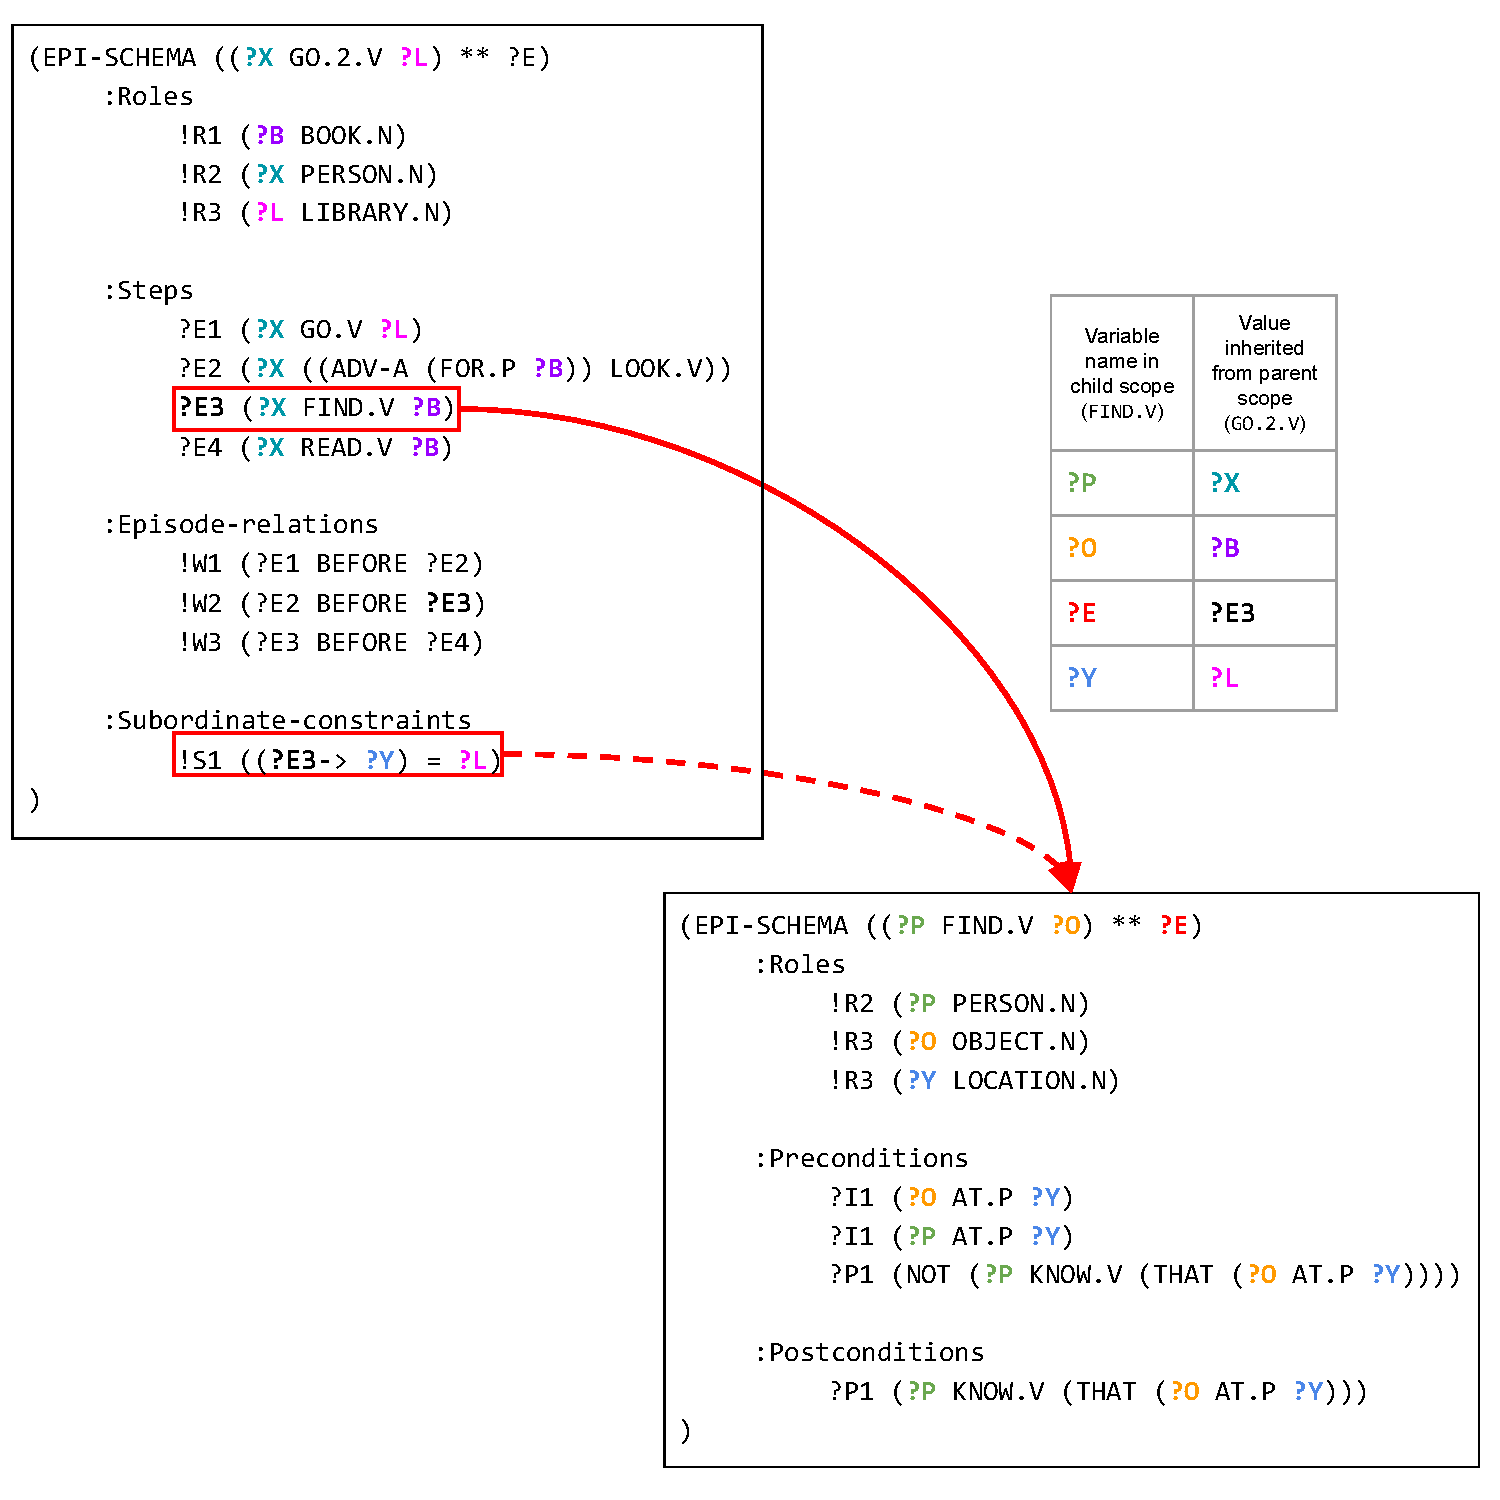
\includegraphics[width=\columnwidth]{CH3_schemas/nesting}
    \caption{An illustration of the \textbf{compositional} hierarchy, in which a \textit{child} schema nested within a \textit{parent}. The child schema \texttt{FIND.V}, shown in the bottom right, is nested within the parent schema \texttt{GO.2.V}, shown in the top left. A table in the upper right shows the new values for the child schema's variables, each inherited from the parent schema.}
    \label{fig:compo_hier}
\end{figure}

\subsection{Specialization Hierarchy}
\begin{figure}
    \centering
    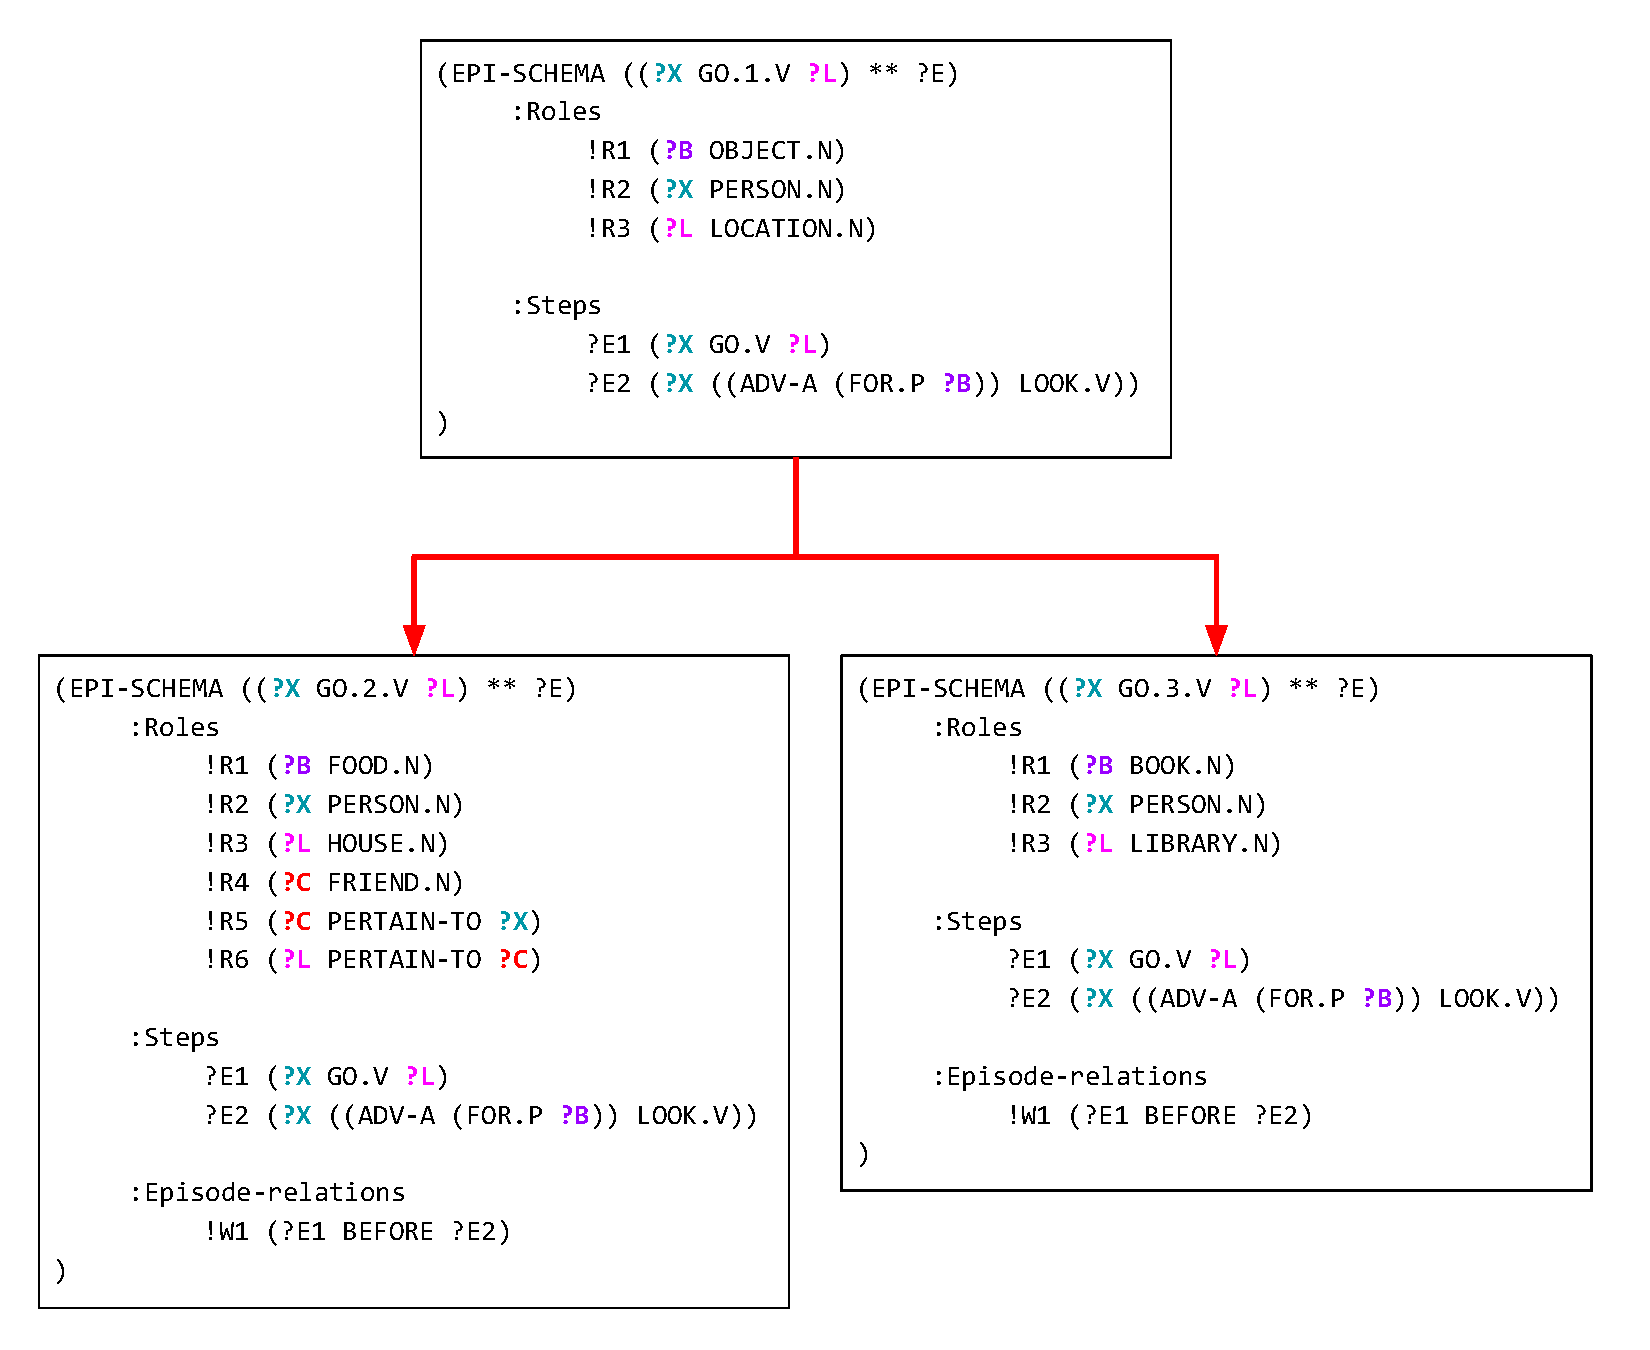
\includegraphics[width=\columnwidth]{CH3_schemas/inheritance}
    \caption{An illustration of the \textbf{specialization} hierarchy, in which two \textit{child} schemas inherit the semantics of a shared \textit{parent}.}
    \label{fig:spec_hier}
\end{figure}
\section{EL Schemas and Formal Semantics}
\label{sec:formal_semantics}
As EL schemas are composed of EL formulas, it is tempting to attempt to specify their full semantics in the model-theoretic terms of EL semantics. It is important to note, however, that the semantics of schema \textit{use}---for matching, inference, and learning---are \textit{not} necessarily well-defined in terms of EL semantics. As an example, consider the decision of whether the invocation a schema $\mathcal{S}$ is ``confirmed'' in an observed story. Some subset of the schema's variables $v \subset vars(\mathcal{S})$ have been bound to individuals in the story, and some subset of the schema's step episodes $e \subset steps(\mathcal{S})$ have been matched to steps in the story. To confirm the invocation of $\mathcal{S}$ and infer the presence of its unobserved formulas, we must map $v$ and $e$ to a truth value in $\{0, 1\}$. Such a function is schema-dependent and can be extremely complex; it likely demands an external heuristic to be practically evaluable, and as such is not explicitly modeled in EL schema semantics. So, while the formulas in an EL schema are interpretable in EL semantics, we must bear in mind that the semantics of the wider schema \textit{system}---which includes matching, inference, and learning---are far more complex, and thus not represented explicitly in the schemas themselves.

Independently of its use or meaning in external systems and procedures, however, a schema can be viewed as a generic statement about the meaning of a kind of event. Much like a gloss uses a generic sentence to define the meaning of a word, an EL schema in its unbound form uses its fluent and non-fluent formulas to define the meaning of its header episode. For example, the schema in Figure~\ref{fig:libschema} purports to generically define what it means for an entity \el{?X}, of type \el{PERSON.N}, to \el{GO.V} to an entity \el{?L}, of type \el{LIBRARY.N}: such an event comprises two steps, \el{?E1} and \el{?E2}, which respectively represent the person's travel to the library and the person's subsequent search for a book. These episodes, the variables in their characterizing formulas, and the types of those variables describe all scenarios \el{?E} wherein a person goes to a library; the predication of their joint truth is a monadic predicate over all episodes, defining what it means to be an episode of a person going to a library. A forward inference rule, in which the predication of joint truth of all schema components implies the schema's header characterization (more or less certainly), and a reverse one, in which the schema's header characterization implies the certainty-weighted truth of all of its components, can be defined within the semantics of EL.

The inference from schema components to the header becomes weaker when based on partial observation, and the semantics becomes murkier. The failure of the example schema to fully describe our intuitive definitions of going-to-the-library events is also an example of the need for continual schema \textit{learning}, the semantics of which are also, as also mentioned above, difficult to render model-theoretically.
%Thus, the remainder of this section will discuss the EL semantics of schemas in this ``tableau'' interpretation, independently of matching, inference, and learning.
\section{Protoschemas}
\label{sec:protoschemas}
What sets our approach to schema learning apart from past approaches is its focus on learning schemas more like a human child does. Human children learn simple schemas like ``sharing toys'' at young ages, but rapidly extend the underlying themes to describe new stereotyped concepts like ``time-shared condominiums'' as they age, by both generalizing out specific fillers like ``toys'', and specifying concepts ``sharing'' to ``time-sharing''. But each schema they learn is a modification to a schema whose overall structure already makes sense to them: the underlying theme of ``sharing'' is really not so different, and might even be inferred from the similarity of the word, or by noticing the similar situation of two people using the same thing. Many of these schemas derive from an initial set of behaviors and tendencies. These initial schemas do not all need to be biologically ``built in'': concepts like sharing are likely learned, but are nevertheless learned quite young. We suggest that the initial set of protoschemas be roughly equivalent to what the average two-year-old child would know, with some examples being:

\begin{enumerate}
    \item Doing something to enable doing something else
    \item Gaining new information
    \item Asking for someone's help to enable doing something
    \item Some basic Schankian ``primitives'': basic knowledge of eating, grasping, sleeping, etc.
\end{enumerate}

%EL schema learning from text is bootstrapped with a set of simple, general schemas---\textit{\textbf{protoschemas}}---that are meant to provide wide coverage of nearly all events and actions represented in texts.
This conceptual ``head start'' mirrors prior knowledge observable even in the youngest humans: young toddlers begin learning about the world in terms of basic actions they already understand quite well, such as the manipulation of objects, the communication of information and requests, and the \textit{use} of those actions in order to attain innate \textit{goals}, like the alleviation of hunger or taking possession of a coveted object. As people age, they acquire schemas detailing progressively more complicated workings of the world, but do so on the basis and in terms of already-known schemas: even situations as complex as global economic supply chain disruptions can generally be understood in terms of basic situation types, e.g. the desire and transportation of objects and the limits of containers.
% Something about how we "cut things off" at 18-24 months to dodge questions of innate-ness
% Cite Piaget
A suitably general set of schemas can, in principle, cover all or most events in English text at some level of generality; even basic generalization of event and action verbs into synonym classes vastly reduces the number of possible linguistic expressions of events. We can further reduce this space with the introduction of a specialization hierarchy and the ability, given that hierarchy, to generalize more specific verbs, e.g. \textit{escape}, into more general verb \textit{classes}, e.g. \textit{movement}.
%Such generalization, of course, comes with information loss, and so, under the fixed constraint that most or all text be understandable, a trade-off is introduced between completeness of initial understanding and manual effort required to craft that initial understanding.

Verbs and verb hierarchies alone do not fully describe the space of even simple events; even when events can be characterized by one verb, the verb's modifiers and arguments must be considered, as well as the types and inter-relations of the arguments. Additionally, information about preconditions, effects, and inherent goals are associated with even basic event types, and can be used to detect implied events in text, e.g. \textit{Jack wanted to win} $\Rightarrow$ \textit{Jack was competing}.
This is why we seek to establish a set of proto-\textit{schemas} to provide head start knowledge.
Single verbs can \textit{represent} most actions and events, though, and thus act as the predicate of EL schema header propositions. With this in mind, we move on to practical investigation of the core question of protoschemas: \textit{how many, and what types, of protoschemas are necessary to bootstrap schema learning from simple texts}?

\subsection{Investigating Protoschema Coverage}
In constructing a set of protoschemas to abstractly cover most or all text during learning, a trade-off must be made between generality and required schema construction effort. On one end of the trade-off, a single, highly general ``something happens'' schema covers all events. On the other end, all verbs require their own manually-constructed schema. To help select a balance point of this trade-off, we investigate the relationship between two corpora: one of existing, hand-written frames, and one of simple child-level stories. We use the FrameNet frame corpus \citep{framenet}, which let us establish two bounds: one upper bound on what amount of manual construction effort is feasible, and one lower bound on the quality and ``interestingness'' of schemas that can be matched to text.
% TODO: describe rocstory corpus here
If many events in the story corpus are unmatchable to FrameNet frames, then the construction of a protoschema corpus may be prohibitively expensive. If most of the events are matchable, however, then it is possible to achieve at least the semantic specificity of FrameNet frames while expending comparable effort.

\subsubsection{Experimental Setup}
Our story set is derived from the ROCstories corpus \citep{mostafazadeh-etal-2016-corpus}. To filter based on conceptual simplicity, we selected a subset of ROCstories for this investigation by sorting all stories by the proportion of their non-stopwords that co-occurred in a set of children's first reader stories \citep{mcguffey}, and then randomly selecting 300 of the 500 stories with the highest such proportions.\footnote{The other 200 were held out for use in \textit{Latent Schema Sampling}, which is discussed in Chapter~\ref{chap:learning}.} To identify the FrameNet frames in this story set, we opted to use a state-of-the-art, neural network-based FrameNet parser, LOME \citep{lome}, as manual annotation on this number of stories was not practical.

As our coverage metric, we evaluated the number of root verbs in the story corpus that invoked FrameNet frames via LOME. To identify the verbs in the corpus, we examined each token's part-of-speech tag using spaCy \citep{spacy2}. After obtaining all frame matches for the corpus, we sorted the matched frame names by the number of verbs they covered, and then re-calculated the coverage metric, for all $K$, using only the top-$K$ most-covering frame names---this gives the marginal value of including each frame. To control for the well-known tendency of a small number of unique verbs to cover a large proportion of verb instances in naturally occurring text \citep{zipf-nl}, we only allowed each frame name to count one match for each unique verb name.

\subsubsection{Results}
Figure~\ref{fig:fn_coverage} shows the results of this experiment. In total, 91\% of all unique verbs in the story corpus were covered by frames identified by LOME. The number of unique frames identified by LOME was 175---far fewer than FrameNet's total number of frames, which exceeds 1,200. Furthermore, even when controlling for the frequency of each verb, a logarithmically increasing relationship between the number of frames used and the number of verbs matched is still apparent, providing further evidence that only a small number of initial frames, or schemas, are necessary to cover most text at FrameNet's average level of generality. The suitability of FrameNet's frames to this task inspired later work on using the LOME FrameNet parser for protoschema identification (see Section~\ref{sec:lome}), as many of our conceptual protoschemas correspond to FrameNet frames.

\begin{figure}
    \centering
    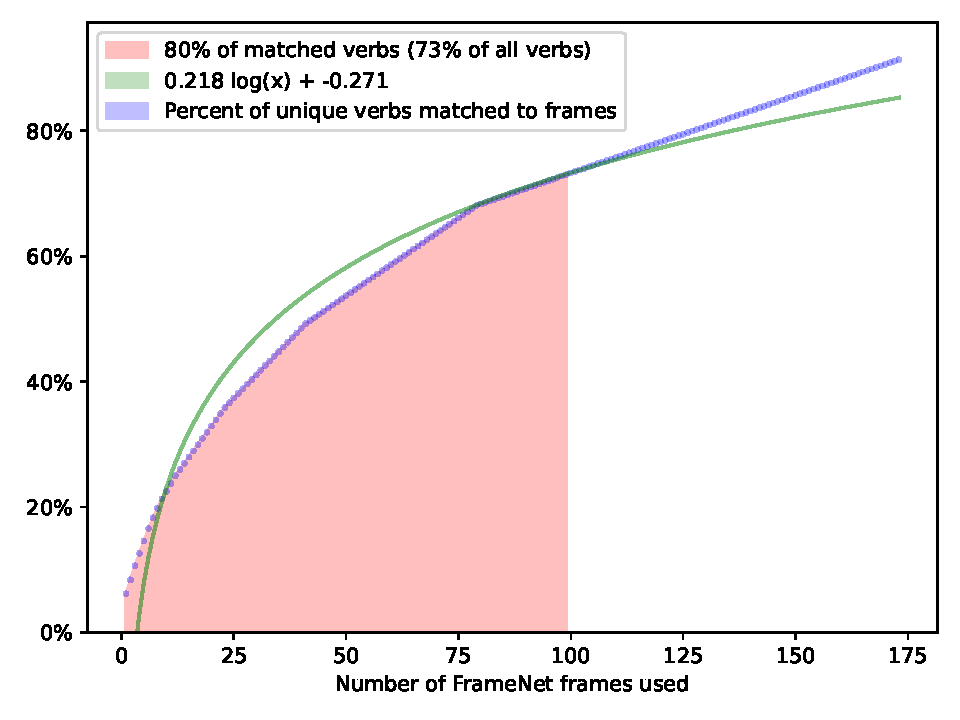
\includegraphics[width=0.75\columnwidth]{CH3_schemas/framenet_coverage}
    \caption{The results of an investigation into the number of verbs in a corpus that can be matched to FrameNet frames. A total of 91\% of verbs can be matched using automated FrameNet matching techniques. The region shaded in red shows that 80\% of all matched verbs can be covered by only 57\% of the total frames invoked across the corpus. The best-fit logarithm is overlaid in green for reference.}
    \label{fig:fn_coverage}
\end{figure}

\section{Matching and Inference}
\label{sec:match_inf}

\textit{Matching} formulas in semantically parsed stories to formulas in schemas underlies both learning and prediction. The formulas comprising a schema are intended to be relatively simple---with complex conjunctions split into separate formulas---and unifiable with formulas parsed from real stories. Unification of a story formula with a schema formula binds individual constants from the former to variables in the latter. These bindings are then substituted in the rest of the schema instance, thereby ``filling in'' some of the missing information. %% I thought the following caveat is needed. -LS
This information is likely to be correct if the story events and participant types matched to the schema can be assumed to provide good evidence for an occurrence of the stereotyped pattern of events the schema captures. 
We refer to any schema instance with one or more bound variables as a \textit{match}.

Using EL formula unification as a primitive, we implement schema matching by iterating through the formulas in an EL parse of a story, matching each formula to any schema formula retrieved as a candidate, and applying the bindings to the schema. When the story has been fully iterated through, or all schema variables have been bound, the match is complete. %% I put in "retrieved as a candidate" -- implying a selective retrieval process. This may not be true right now, but will be essential for scaling up.

We randomly permute story formulas and unify them, in the randomized order, with schema formulas.
%% Actually I'm not quite sure what this means or how defensible it is. Why not match each episodic story formula, along with any available argument type constraints, to each episodic schema formula, registering the quality of each match (where "more specific" implies higher quality), and then use those match data to do a greedy search for a "best subset of matches" (e.g., start with the one or two best matches, bind variables accordingly, then see if you can add more matches with "good enough" match scores under the same (or compatible) bindings?
We try multiple permutations to explore the space of possible matches, and cache low-level unification results to speed up the process.

\begin{algorithm}
\caption{Basic algorithm for matching a story to a schema}
\label{alg:matching}
\begin{algorithmic}
\STATE INPUT: set of story EL formulas $STORY$, a candidate schema $SCH$, number of shuffles $SHUF$, match scoring function $score$
\STATE OUTPUT: best schema $match$
\STATE $match \gets null$
\FOR{i from 0 to $SHUF$}
    \STATE $STORY \gets shuffle(STORY)$
    \FOR{$\phi$ in $STORY$}
        \FOR{$\psi$ in $SCH$}
            \IF{$\phi$ and $\psi$ unify with variable bindings $B$}
                \STATE $SCH \gets SCH$ with all bindings in $B$ applied
            \ENDIF
        \ENDFOR
    \ENDFOR
    \IF{$score(SCH) > score(match)$}
        \STATE $match \gets SCH$
    \ENDIF
\ENDFOR
\end{algorithmic}
\end{algorithm}

\subsection{Generalizing Matches}
To generalize a match into a new, ``learned'' schema, we need to incorporate incidental information about the matched value. For example, the variables of the \texttt{travel.v} protoschema can be bound by the constants in the formula \texttt{((MONKEY27.SK (CLIMB.V TREE28.SK)) ** E34.SK)} in a story about a monkey climbing a tree, but re-generalizing the constants \texttt{MONKEY27.SK} and \texttt{TREE28.SK} into unconstrained variables would remove all the information we learned. However, if we incorporate formulas about the types of those objects into our new schema---such as the formulas \texttt{(MONKEY27.SK MONKEY.N)} and \texttt{(TREE28.SK TREE.N)}---we can then generalize the constants but maintain knowledge of their types.

\subsection{Learning Composite Schemas}
If schemas could only be learned by progressively refining existing protoschemas, schemas would mostly be single-step actions. Some of these, like ``monkey eats banana'', would still be valuable world knowledge, but many more complex event patterns would not be learnable. However, our schema formalism allows for multiple steps, and allow for subschemas within them as steps; we would like to be able to learn schemas that make use of that complexity.

\textit{``First-order''} schemas---that is, refinements of our starting protoschemas---can be strung together into composite schemas in multiple ways. If a schema B has a precondition that unifies with one of schema A's postconditions, and schema A's episode is temporally before schema B's, the two can be ``chained'' together; these chains can be further extended by other simple schemas. This chaining process was how the system learned the schema in Figure~\ref{fig:eg_schema}. Goals may also be unified with postconditions to establish chains.


%\subsection{Certainties}


\iffalse
In this chapter, we describe the schema representation we've developed, the idea of the ``protoschema approach'' to schema learning, and the system we've implemented to perform story parsing and schema learning.

\section{Schema Representation}
A knowledge base used for story understanding should be computationally manipulable and facilitate powerful inference procedures. Past approaches, like those described in Chapter~\ref{ch:bg}, have made use of either simplified tuple event representations or FOL-based logical representations with poor expressiveness. Our EL-based schema system maintains a form similar in expressive capacity to natural language, while still offering representational features not found in existing schema learning systems, such as inter-related entity slots, complex temporal relationships between events, schemas embedded as steps within other schemas, and probabilistic certainty scores for constraints.

In this section, we will describe our schema model, examples of which can be seen in Figures \ref{fig:protoschema}, \ref{fig:schema_match}, and \ref{fig:eg_schema}. Our schemas are formulated in terms of Episodic Logic (EL) formulas, organized into sections. We describe the sections below.

\subsection{Overall Structure}
A schema is represented by its \textit{header}, seen in line 1 of Figure~\ref{fig:eg_schema}. A schema's header is an EL proposition and an episode characterized by the proposition, here \texttt{?E}. The header episode summarizes the entire schema. This can be used to ``embed'' a schema as a step in another schema---in fact, each step in Figure~\ref{fig:eg_schema} is a header for an embedded schema---or it can be matched directly to a proposition in a story to automatically invoke the schema.

The rest of the schema is laid out in two types of sections: \textit{fluent} and \textit{nonfluent} sections. Nonfluent sections such as \texttt{Roles} and \texttt{Episode-relations}, whose formula IDs all begin with exclamation marks, contain formulas that hold true regardless of time. Fluent sections, such as \texttt{Steps} and \texttt{Preconds}, contain formulas identified by variables starting with question marks; these formulas are susceptible to change over time. We will now examine these sections, and what they're used for, in more detail.

\subsection{Roles}
The \textbf{Roles} section of a schema is a \textit{nonfluent} section meant for putting ``eternal'' type constraints on the participating entities in the schema. All of the schema's variables, starting with question marks, can be viewed as Skolem functions of the schema's header episode, and they can be constrained in this section. In addition to type constraints, e.g. \texttt{(?X DOG.N)}, relational constraints between entities can also be specified in this section, e.g. \texttt{(?X PERTAINS\_TO.N ?Y)}.
%%, and they can be constrained in this section.
%% Not clear what this means -- you've already mentioned type constraints; do you mean to refer to other nonfluent contraints here? -LS
%% L: I've added a mention of relational constraints in addition to type constraints.

In Figure~\ref{fig:protoschema}, the protoschema for movement from location to location, there are three main participating entities: \texttt{?X}, the agent doing the movement, and \texttt{?L1} and \texttt{?L2}, the source and destination locations. Those ``types'' are EL predicates, and are enforced by the predications in the protoschemas \textbf{Roles} section.

When formulas are unified with a schema, these formulas are used as constraints for evaluating whether the individuals bound to the variables satisfy the schema's semantics. They are evaluated in a knowledge base populated by facts from the story, and potentially by formulas predicted from other confirmed schema matches. Partial matches, or matches with partial constraint satisfaction, can still be valuable: ``Breaking the mold'' of known schemas is part of the learning process. More detail on constraint evaluation and scoring will be given in Section~\ref{sec:scoring}.
%% Minor US stylistic convention: Start with capitalized word after a colon, iff the material after the colon is a complete sentence.

\subsection{Preconditions, Postconditions, and Goals}
Actions undertaken in the real world are frequently goal-driven, and a representation of how actions change the world and why characters might perform them is necessary to understand the story. The episodes characterized by the formulas in the precondition section are tacitly assumed to start before the schema's header episode (adjoining or overlapping it), and those characterized in the postcondition section extend beyond the header episode (post-adjoining or overlapping it).
%% Lane, we've mulled over the above temporal relations before, and I had conceded that it's ok to say the precond episodes immediately precede the header episode, while the postcond episodes immediately follow it; overlap isn't precluded in the sense that those precond & postcond episodes may be parts of larger episodes of the same type. However, on further thought, this view of preconds and postconds could lead to contradiction for multistep schemas. For example, consider making toast with peanut butter, requiring toasting the piece of bread and then spreading peanut butter on it. The goal state is that we have the piece of bread in a "toasted" state, with peanut butter on it. However, The bread should be in a "toasted" state already when we spread the peanut butter, and we may well wish to assert that constraint. But if we take it to be implicitly true that the postcondition, say ?e4, corresponding to the toasted state starts at the end of the overall schema episode, we can't consistently assert a constraint that it starts right after the toasting episode.
%% L: I suppose I don't see a problem: the ``default'' constraints on the postconditions of 1. toastedness and 2. peanut-butteriness would say that both postconditions become true at some point during the schema episode, and are true immediately after the schema episode. Further constraints could be added as episode relations, saying that postcondition 1 is true at the start of postcondition 2.

Schema matches can be ``chained together'' into composite, multi-step schemas by unifying their pre- and post-conditions, or their goals and post-conditions. An example of a learned ``chained'' schema is given in Figure~\ref{fig:eg_schema}.

\subsection{Temporal Relations}
Schemas characterize EL episodes that encompass their temporal duration. They also contain many other episodes, such as steps and preconditions, with their own temporal bounds. These episodes can all be complexly inter-related using constraints from the Allen Interval Algebra \citep{allen1983maintaining}. Pre- and post-conditions are implicitly constrained to be true at the start and end of the schema's header episode, respectively, and steps, by default, are ordered sequentially as listed in the schema, but additional constraints can be specified in the \textbf{Episode-relations} section of each schema. To evaluate these interval constraint propositions, we implemented a time graph specialist module \citep{gerevini1993efficient}.


\section{Schema Learning}
\label{sec:learning}
In this section, we describe how our system learns new schemas from natural language stories. We describe our parsing process for natural language stories, the process of matching parsed stories to schemas, how schema matches can be generalized to create new schemas, and how partial schema matches can be used to predict events in similar stories with missing details.

\subsection{The Protoschema Approach}
As noted, generate new schemas from stories by starting with an initial set of \textit{protoschemas} that we would expect a 1- or 2-year-old child to have; these encode very general knowledge about physical and communicative actions, with their preconditions and effects. Examples of protoschemas we've already written include movement of an agent from one location to another (Figure~\ref{fig:protoschema}), consumption of food, and possession and transfer of possession.
These protoschemas are then invoked by actions in stories---for example, the ``travel'' protoschema in Figure~\ref{fig:protoschema} matched a ``climb'' action in the story in Figure~\ref{fig:story} to yield a ``monkey climbs a tree'' schema, shown in Figure~\ref{fig:schema_match}. \footnote{``travel'' was invoked by ``climb'' by way of the WordNet hypernym hierarchy.}

\subsection{Story Parsing}
\label{sec:parsing}
Formulas in schemas are represented in Episodic Logic, and can only be matched to other EL formulas. We have developed a stage-based parser to convert stories into EL formulas ready to be matched with schemas. In the first stage, the raw story text is run through the AllenNLP co-reference analyzer \citep{Gardner2017AllenNLP}, and co-referring word spans are tagged with entity numbers. The text is then parsed by the BLLIP parser \citep{charniak2000maximum}, the output of which is transduced into \textit{Underspecified Logical Form} (ULF) \citep{kim2019IWCS}, an underspecified variant of EL without scoped quantifiers or temporally de-indexed tenses. A series of transduction rules then converts the ULF to full EL, splitting complex formulas into conjunctions of simpler ones to facilitate ``piecewise'' matching with the short formulas in schemas.

\subsection{Matching}

\textit{Matching} formulas in semantically parsed stories to formulas in schemas underlies both learning and prediction. The formulas comprising a schema are intended to be relatively simple---with complex conjunctions split into separate formulas---and unifiable with formulas parsed from real stories. Unification of a story formula with a schema formula binds individual constants from the former to variables in the latter. These bindings are then substituted in the rest of the schema instance, thereby ``filling in'' some of the missing information. %% I thought the following caveat is needed. -LS
This information is likely to be correct if one or more story formulas matched to the same schema are apt to indicate the occurrence of the kind of pattern of events the schema captures. 
We refer to any schema instance with one or more bound variables as a \textit{match}.

Using EL formula unification as a primitive, we implement schema matching roughly according to Algorithm~\ref{alg:matching}. In its simplest form, the algorithm iterates through the formulas in an EL parse of a story, matching each formula to any schema formula it can and applying the bindings to the schema. When the story has been fully examined, the match is complete.

However, the order of matched formulas matters: for example, if there are two agent slots in an ``X feeds Y'' schema, we may match the first suitable agent we see in the story to X, and that binding would persist for the remainder of the matching process, even if Y may have been a better option. To address this, we ``shuffle'' each story's EL formulas some number of times, and repeat the matching algorithm, stochastically pursuing a better match. With efficient caching of lower level unification operations, this turns out to be a fairly efficient way to explore the match space of a story and a schema.

\subsubsection{Partial Matches and Scoring}
\label{sec:scoring}

When a schema is matched to a story, some constraints may be broken; this is a natural part of the learning process. A schema for a cow eating grass matching to a story about a dog eating grass violates the cow constraint on a participating entity, but is a valuable source of knowledge if properly generalized. On the other hand, too many broken constraints are indicative of a poor match between a schema candidate and a story.

Schema matches are essentially scored by counting satisfied constraints, with some added complexity. For example, nonfluent Role constraints are worth half as many points as fluent events in the Steps section that have been matched to the story---intuitively, a full event is a stronger signal than a property of an entity. Confirming the schema's header formula is worth twice the points of any other event.

For inexact matches---e.g. \texttt{(?X COW.N)} and \texttt{(ROVER.NAME DOG.N)}---the score of the binding is further weighted by the approximate semantic similarity of the two words. If one subsumes the other on a hypernym hierarchy, the strength is scaled by the distance of the two in that hierarchy. If neither subsumes the other, but they share a common ancestor hypernym, the strength is half their average distance to that ancestor.

The hypernym score accounts for half of the overall weight of an inexact match; the other half is provided by their semantic similarity according to a pre-trained word embedding model. \footnote{\textit{GoogleNews-vectors-negative300.bin}, \citet{NIPS2013_5021}}


\subsection{Generalizing Matches}
To generalize a match into a new, ``learned'' schema, we need to incorporate incidental information about the matched value. For example, the variables of the \texttt{travel.v} protoschema in Figure~\ref{fig:protoschema} can be bound by the constants in the formula \texttt{((MONKEY27.SK (CLIMB.V TREE28.SK)) ** E34.SK)} in the story in Figure~\ref{fig:story_parse}, but re-generalizing the constants \texttt{MONKEY27.SK} and \texttt{TREE28.SK} into variables would remove all the information we learned. However, if we incorporate formulas about the types of those objects into our new schema---like the formulas \texttt{(MONKEY27.SK MONKEY.N)} and \texttt{(TREE28.SK TREE.N)}---we can then generalize the constants but maintain knowledge of their types.

\subsubsection{Re-Matching Learned Schemas}

Once a protoschema has been matched to a story and generalized into a learned schema, it may contain extraneous details or overly specific constraints. However, the space of possible generalizations is large: if there are N constraints with even only one possible generalization each, like \texttt{DOG.N} and \texttt{ANIMAL.N}, the possible generalizations of the entire schema number $2^N$.

To learn reasonable generalizations of learned schemas, we can simply continue our matching process by adding them to the set of initially known schemas, alongside the protoschemas. If they are retrieved as candidates and receive high match scores for another story, shared details of each match can more certainly be incorporated into a general schema.

For example, Figure~\ref{fig:rematch_1} is a ``first-order'' schema derived from a match of an eating protoschema with the sentence ``the cow ate the grass''. When matched to the similar sentence ``the dog ate the grass'', we derive the ``second-order'' schema in Figure~\ref{fig:rematch_2}. Note that \texttt{DOG.N} and \texttt{COW.N} have been automatically generalized, via the WordNet hypernym hierarchy, to \texttt{PLACENTAL.N}. The former two constraints remain in the schema, albeit at a lower \textit{certainty} score of $1/2$ each. The latter general constraint has a higher certainty of $2/2$. These correspond to the frequency of observance in all stories that have contributed to the learned schema.

\subsection{Learning Composite Schemas}
If schemas could only be learned by progressively refining existing protoschemas, schemas would mostly be single-step actions. Some of those, like ``monkey eats banana'', would still be valuable world knowledge, but many situations would not be learnable. Our schemas can have multiple steps, however, and even nest other schemas within them as steps; we would like to be able to learn schemas that make use of that complexity.

\textit{``First-order''} schemas---that is, refinements of our starting protoschemas---can be strung together into composite schemas in multiple ways. If a schema B has a pre-condition that unifies with one of schema A's post-conditions, and schema A's episode is temporally before schema B's, the two can be ``chained'' together; these chains can be further extended by other simple schemas. This chaining process was how the system learned the schema in Figure~\ref{fig:eg_schema}. Goals may also be unified with post-conditions to establish chains.

\subsection{Prediction}
Prediction is relatively straightforward: Given a story, such as the one in Figure~\ref{fig:predictions}, we try to identify a similar schema, such as the learned schema in Figure~\ref{fig:eg_schema}, and match as many formulas as we can to it. After we've substituted story entities for variables, we may fill in other formulas in the schema. Schema formulas whose variables have all been filled in, but are not present in the story, are predictions: we guess that the schema underlies the observed events, and infer the rest of the situation from what we know.

\begin{figure}[htbp]
    \begin{lstlisting}[frame=single,numbers=left,numberstyle=\tiny,xleftmargin=1.5em,style=Schemas]
(EPI-SCHEMA ((?X_D EAT.379.V ?X_C)
                ** ?X_E)
	:ROLES
		!R1 (?X_D AGENT.N)
		!R2 (?X_C FOOD.N)
		!R3 (?X_C GRASS.N)
		!R4 (?X_D COW.N)
	:GOALS
		?G1 (?X_D (WANT.V (THAT (NOT
		    (?X_D HUNGRY.A)))))
	:PRECONDS
		?I1 (?X_D HAVE.V ?X_C)
		?I2 (?X_D HUNGRY.A)
	:POSTCONDS
		?P1 (NOT (?X_D (HAVE.V ?X_C)))
		?P2 (NOT (?X_D HUNGRY.A))
	:EPISODE-RELATIONS
		!W1 (?P1 AFTER ?X_E)
		!W2 (?I1 BEFORE ?X_E)
	:NECESSITIES
		!N1 (!R1 NECESSARY-TO-DEGREE 1.0)
)
)\end{lstlisting}
    \caption{A schema learned by applying the eating protoschema to the sentence ``the cow ate the grass''.}
    \label{fig:rematch_1}
\end{figure}

\begin{figure}[htbp]
    \begin{lstlisting}[frame=single,numbers=left,numberstyle=\tiny,xleftmargin=1.5em,style=Schemas]
(EPI-SCHEMA ((?X_D EAT.7.V ?X_C)**?X_E)
	:ROLES
		!R1 (?X_D AGENT.N)
		!R2 (?X_C FOOD.N)
		!R3 (?X_D COW.N)
		!R6 (?X_C GRASS.N)
		!R7 (?X_D DOG.N)
		!R8 (?X_D PLACENTAL.N)
	:GOALS
		?G1 (?X_D (WANT.V (THAT (NOT
		        (?X_D HUNGRY.A)))))
	:PRECONDS
		?I1 (?X_D HAVE.V ?X_C)
		?I2 (?X_D HUNGRY.A)
	:POSTCONDS
		?P1 (NOT (?X_D (HAVE.V ?X_C)))
		?P2 (NOT (?X_D HUNGRY.A))
	:EPISODE-RELATIONS
		!W1 (?P1 AFTER ?X_E)
		!W2 (?I1 BEFORE ?X_E)
	:CERTAINTIES
		!C1 (!R8 CERTAIN-TO-DEGREE (/ 2 2))
		!C2 (!R3 CERTAIN-TO-DEGREE (/ 1 2))
		!C3 (!R7 CERTAIN-TO-DEGREE (/ 1 2))
	:NECESSITIES
		!N1 (!R1 NECESSARY-TO-DEGREE 1.0)
)
)\end{lstlisting}
    \caption{A more general schema learned by applying the learned schema in Figure~\ref{fig:rematch_1} to the sentence ``the dog ate the grass''.}
    \label{fig:rematch_2}
\end{figure}

\begin{algorithm}
\caption{Basic algorithm for matching a story to a schema}
\label{alg:matching}
\begin{algorithmic}
\STATE INPUT: set of story EL formulas $STORY$, a candidate schema $SCH$, number of shuffles $SHUF$
\STATE OUTPUT: best schema $match$
\STATE $match \gets null$
\FOR{i from 0 to $SHUF$}
    \STATE $STORY \gets shuffle(STORY)$
    \FOR{$\phi$ in $STORY$}
        \FOR{$\psi$ in $SCH$}
            \IF{$\phi$ and $\psi$ unify with variable bindings $B$}
                \STATE $SCH \gets SCH$ with all bindings in $B$ applied
            \ENDIF
        \ENDFOR
    \ENDFOR
    \IF{$score(SCH) > score(match)$}
        \STATE $match \gets SCH$
    \ENDIF
\ENDFOR
\end{algorithmic}
\end{algorithm}

\begin{figure}[htbp]
        \begin{lstlisting}[frame=single,numbers=left,numberstyle=\tiny,xleftmargin=1.5em,style=Schemas]
The monkey can climb a tree.
He climbs the tree and gets a cocoanut.
He drops the cocoanut to the ground.
He comes down and eats it.\end{lstlisting}
    \caption{An example of a children's story used as input to our system for schema learning.}
    \label{fig:story}
\end{figure}

\begin{figure}[htbp]
        \begin{lstlisting}[frame=single,numbers=left,numberstyle=\tiny,xleftmargin=1.5em,style=Schemas]
(TREE28.SK TREE.N)
(MONKEY27.SK MONKEY.N)
((MONKEY27.SK((CAN.MD CLIMB.V)
    TREE28.SK))**E26.SK)
((MONKEY27.SK (CLIMB.V TREE28.SK))
    ** E34.SK)
((MONKEY27.SK (GET.V COCOANUT32.SK))
    ** E33.SK)
(COCOANUT32.SK COCOANUT.N)
(TREE28.SK TREE.N)
(GROUND39.SK GROUND.N)
((MONKEY27.SK (DROP.V COCOANUT32.SK))
    ** E40.SK)
(COCOANUT32.SK COCOANUT.N)
((MONKEY27.SK (EAT.V COCOANUT32.SK))
    ** E44.SK)\end{lstlisting}
    \caption{The story in Figure~\ref{fig:story} parsed into Episodic Logic}
    \label{fig:story_parse}
\end{figure}

\begin{figure}[htbp]
    \begin{lstlisting}[frame=single,numbers=left,numberstyle=\tiny,xleftmargin=1.5em,style=Schemas]
(EPI-SCHEMA((?X TRAVEL.V
    (FROM.P-ARG ?L1) ?L2)**?E)
  :ROLES
    !R1 (?X AGENT.N)
    !R2 (?L1 LOCATION.N)
    !R3 (?L2 LOCATION.N)
  :GOALS
    ?G1 (?X (WANT.V
               (KA ((ADV-A (AT.P ?L2))
                BE.V))))
  :PRECONDS
    ?I1 (?X (AT.P ?L1))
    ?I2 (NOT (?X (AT.P ?L2)))
  :POSTCONDS
    ?P1 (NOT (?X (AT.P ?L1)))
    ?P2 (?X (AT.P ?L2))
  :NECESSITIES
    !N1 (!R1 NECESSARY-TO-DEGREE 1.0)
)\end{lstlisting}
    \caption{An example of a \textit{protoschema}: a general schema used to ``bootstrap'' the system and generate more specific schemas.}
    \label{fig:protoschema}
\end{figure}

\begin{figure}[htbp]
    \begin{lstlisting}[frame=single,numbers=left,numberstyle=\tiny,xleftmargin=1.5em,style=Schemas]
(EPI-SCHEMA ((?X_B CLIMB.481.V
                (FROM.P-ARG ?L1) ?X_C)
                    ** ?X_E)
  :ROLES
    !R1 (?X_B AGENT.N)
    !R2 (?L1 LOCATION.N)
    !R3 (?X_C LOCATION.N)
    !R4 (?X_C TREE.N)
    !R5 (?X_B MONKEY.N)
  :GOALS
    ?G1 (?X_B (WANT.V
                (KA ((ADV-A
                (AT.P ?X_C)) BE.V))))
  :PRECONDS
    ?I1 (?X_B (AT.P ?L1))
    ?I2 (NOT (?X_B (AT.P ?X_C)))
  :POSTCONDS
    ?P1 (NOT (?X_B (AT.P ?L1)))
    ?P2 (?X_B (AT.P ?X_C))
  :NECESSITIES
    !N1 (!R1 NECESSARY-TO-DEGREE 1.0)
)\end{lstlisting}
    \caption{A schema match of the story in Figure~\ref{fig:story} to the protoschema in Figure~\ref{fig:protoschema}}
    \label{fig:schema_match}
\end{figure}

\begin{figure}[htbp]
    \begin{lstlisting}[frame=single,numbers=left,numberstyle=\tiny,xleftmargin=1.5em,style=Schemas]
(EPI-SCHEMA ((?X_B CLIMB_GET_EAT.PR
                ?X_A ?X_C) ** ?E)
  :ROLES
    !R1 (?X_A TREE.N)
    !R2 (?X_C INANIMATE_OBJECT.N)
    !R3 (?X_B MONKEY.N)
    !R4 (?X_C FOOD.N)
    !R5 (?X_C COCOANUT.N)
  :STEPS
    ?E1 (?X_B CLIMB.481.V
            (FROM.P-ARG ?L1) ?X_A)
    ?E2 (?X_B GET.511.V ?X_C
            (AT.P-ARG ?X_A))
    ?E3 (?X_B EAT.541.V ?X_C)
  :EPISODE-RELATIONS
    !W1 (?E1 BEFORE ?E2)
    !W2 (?E2 BEFORE ?E3)
    !W3 (?E1 DURING ?E)
    !W4 (?E2 DURING ?E)
    !W5 (?E3 DURING ?E)
)\end{lstlisting}
    \caption{An example of a multi-step schema learned by our system from protoschema matches to the story in Figure~\ref{fig:story}}
    \label{fig:eg_schema}
\end{figure}

\lstdefinestyle{Schemas2}{
morekeywords={prediction},
basicstyle=\ttfamily\footnotesize\bfseries,
stringstyle=\ttfamily\color{stringcolor},
commentstyle=\ttfamily\color{commentcolor},
keywordstyle=\ttfamily\color{stringcolor},
identifierstyle=\texttt,
tabsize=2
}

\begin{figure}[htbp]
    \begin{lstlisting}[frame=single,numbers=left,numberstyle=\tiny,xleftmargin=1.5em,style=Schemas2]
The cocoanut tree is tall.
It is very pretty.
Many cocoanuts grow on the tree.
Simeon can climb the tree.
prediction:
   (SIMEON.NAME MONKEY.N)
prediction:
   (TREE1604.SK ((NN COCOANUT.N) TREE.N))
prediction:
    (SIMEON.NAME CLIMB.481.V TREE1604.SK)
He gets the cocoanuts for his mother.
prediction:
    (SIMEON.NAME EAT.541.V COCOANUT1626.SK)
His mother likes cocoanuts.
She likes to play with Simeon.\end{lstlisting}
    \caption{Another children's story, interspersed with predictions made by matching its parse to the learned schema in Figure~\ref{fig:eg_schema}}
    \label{fig:predictions}
\end{figure}
\fi
